% @Author: AnthonyKenny98
% @Date:   2020-04-07 11:00:50
% @Last Modified by:   AnthonyKenny98
% @Last Modified time: 2020-04-10 15:04:02
\begin{figure}[H]
\begin{centering}
\begin{tabular}{cc}
    \begin{subfigure}{0.47\linewidth}
    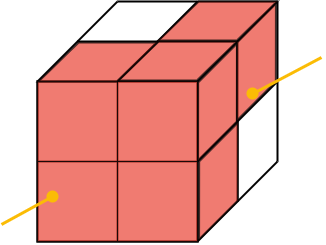
\includegraphics[width=\linewidth]{chapters/chapter3/img/edge_collision_planes_a.png}
    \caption{}
    \label{fig:edge_collision_planes_a}
    \end{subfigure} &

    \begin{subfigure}{0.47\linewidth}
    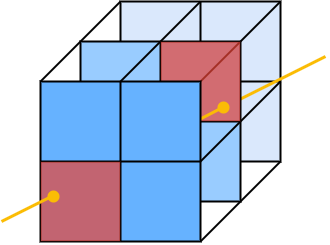
\includegraphics[width=\linewidth]{chapters/chapter3/img/edge_collision_planes_b.png}
    \caption{}
    \label{fig:edge_collision_planes_b}
    \end{subfigure} \\

    \begin{subfigure}{0.47\linewidth}
    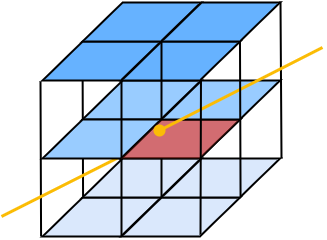
\includegraphics[width=\linewidth]{chapters/chapter3/img/edge_collision_planes_c.png}
    \caption{}
    \label{fig:edge_collision_planes_c}
    \end{subfigure} &

    \begin{subfigure}{0.47\linewidth}
    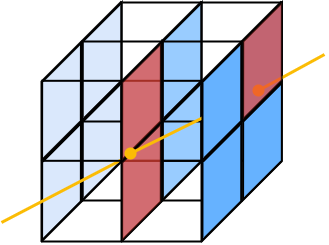
\includegraphics[width=\linewidth]{chapters/chapter3/img/edge_collision_planes_d.png}
    \caption{}
    \label{fig:edge_collision_planes_d}
    \end{subfigure} \\
\end{tabular}

\mycaption{Detecting Grid Intersections by Finding Intersections with Axis Oriented Planes}{\\ Consider an edge $e$ that spans the width of a $2\times 2\times 2$ grid map, as shown in Figure \ref{fig:edge_collision_planes} (do not consider if the grids are occupied, this is just to determine which of them the edge intersects). Just by eyeballing Figure \ref{fig:edge_collision_planes_a} it seems odd that so many of the grids have been intersected (denoted by red shading) by the yellow edge. The algorithm executes by checking one set of \glspl{axis-oriented plane} at a time. Figure \ref{fig:edge_collision_planes_a} shows how the $xy$-oriented planes are checked for 3 different values of $z$ (going into the page), finding two intersection points. There is only one intersection for the $xz$ oriented planes (\ref{fig:edge_collision_planes_c}). In Figure \ref{fig:edge_collision_planes_d}, the segment intersects 2 grids in the second $yz$-oriented plane, and one in the third plane. The intersected grids are thus any grid where a point-of-intersection falls on its face.}
\label{fig:edge_collision_planes}
\end{centering}
\end{figure}